\documentclass[10pt,xcolor=dvipsnames]{beamer}
\usepackage{graphicx}
\usepackage{multimedia}
\usepackage{epsf,amsmath,amssymb,amsfonts}
\usetheme{CambridgeUS}

%---------------------------------------------------------------------------
%
%          USER DEFINED MACROS
%
%\mathsurround = 2pt

\def \ds          {\displaystyle}
\def \rmd         {{\rm d}}
\def \be          {{\bf e}}
\def \bF          {{\bf F}}
\def \bI          {{\bf I}}
\def \bn          {{\bf n}}
\def \bff         {{\bf f}}
\def \bdf         {{\bf df}}
\def \bdT         {{\bf dT}}
\def \bT          {{\bf T}}
\def \cT          {{\cal T}}
\def \bU          {{\bf U}}
\def \bu          {{\bf u}}
\def \bv          {{\bf v}}
\def \bV          {{\bf V}}
\def \bX          {{\bf X}}
\def \by          {{\bf y}}
\def \bY          {{\bf Y}}
\def \bz          {{\bf z}}
\def \bZ          {{\bf Z}}
\def \bW          {{\bf W}}
\def \bZt         {{\bf \widetilde Z}}
\def \bzi         {{\bz}_i}
\def \bzs         {{\bz}^*}
\def \bzis        {{\bz}_i^*}
\def \bzin        {\{\bzi\}_{i=1}^k}
\def \cf          {{\cal F}}
\def \cg          {{\cal G}}
\def \ch          {{\cal H}}
\def \vi          {{V_i}}
\def \vin         {\{\vi\}_{i=1}^k}
\def \Babs        {{\Big|}}
\def \Bl          {{\Big(}}
\def \Br          {{\Big)}}
\def \Bleft       {{\Big[}}
\def \Bright      {{\Big]}}
\def \p           {\partial}
\def \R           {{\mathbb R}}
\def \N           {{\mathbb N}}
\def\y            {{\bf y}}
\def \tN          {{\widetilde{N}}}
\def \tD          {{\widetilde{D}}}

\def \proofnote #1{\footnote{{\bf Note: #1}}}
\def \norm      #1{\left\|\,#1\,\right\|}
\def \set       #1{\left\{\,#1\,\right\}}
\def \tr          {^T}
\def \IhH         {I_h^H}
\def \IhHb        {{\hat I}_h^H}
\def \IHh         {I_H^h}
\def \vbar        {\bar v}
\def \zhbar       {\bar z_h}
\def \zHbar       {\bar z_H}
\def \zhplus      {z_h^+}
\def \zHplus      {z_H^+}

\renewcommand{\theequation}{\thesection.\arabic{equation}}

\newtheorem{alg}{Algorithm}[section]
\newtheorem{thm}{Theorem}[section]
\newtheorem{lem}[thm]{Lemma}
\newtheorem{cor}[thm]{Corollary}
\newtheorem{pro}{Proposition}[section]
\newtheorem{defn}{Definition}[section]
\newtheorem{asp}{Assumption}[section]
\newtheorem{rmk}{Remark}[section]

%\def \Rblack#1{\,\hbox{R \kern-1.2em I
%    \kern.275em $^{#1}$}}
%\def \bG{{\bf G}}
%\def \bt{{\bf t}}
%\def \bzj{{\bz}_j}
%\def \bY{{\bf Y}}
%\def \byi{{\by}_i}
%\def \byj{{\by}_j}
%\def \byim{\{\byi\}_{i=1}^m}
%\def \bx{{\bf x}} 


\author[Zichao Di]{Zichao Di\\ {\footnotesize Department of Mathematical Sciences\\ George Mason University}\\
\quad \quad \\ \quad \quad \\ 
{\footnotesize Joint work with:\\ Maria Emelianenko \\Stephen G. Nash}}
%\author [Advisors: Maria Emelianenko\\  Stephen G. Nash]

\title[MG/OPT method for CVTs]{Novel Optimization-based Multilevel CVT \\Construction Algorithm }
\date{July 22, 2011}
\institute[George Mason University]{}
\setbeamertemplate{navigation symbols}{}
\begin{document}
\frame{\titlepage}
%%%%%%%%%%%%%%%%%%%%%%%%%%%%%%%%%%%%%%


\section{Outline}
\subsection{Outline}
\frame{
\frametitle{Outline}
\begin{itemize}
\item{\em Introduction}
\begin{itemize}
\item Centroidal Voronoi tessellation (CVT) formulation
\end{itemize}


\item{\em Multigrid-based Optimization for CVT construction}
\begin{itemize}
\item Multigrid Optimization (MG/OPT) algorithm: background
\item Applying MG/OPT to the CVT Formulation
\end{itemize}

\item Numerical Experiments
\begin{itemize}
\item 1-dimensional examples
\item 2-dimensional examples
\end{itemize}

\item Comments and Conclusions
\end{itemize}
}
%%%%%%%%%%%%%%%%%%%%%%%%%%%%%%%%%


\section{CVT background}
\subsection{Introduction}
\frame{
\frametitle{Centroidal Voronoi tessellation (CVT)}
\begin{columns}
\column{3in}
\begin{itemize}
\item Given 
\begin{itemize}
\item a set of points $\{\bzi\}_{i=1}^{k}$ (generators)
\item a set of regions $\{V_i\}_{i=1}^{k}$ (Voronoi tessellation)
\end{itemize}
\item Define {\color{blue} {\em the centroids}}: $\quad \bzi^{*}=\frac{\displaystyle \int_{V_{i}}\rho(y)y dy}{\displaystyle \int_{V_i}\rho(y) dy}$
\item Define  {\color{blue} {\em energy functional}}: $$ \label{ener}
{\cg}\Bigl(\bzin\Bigr)
=
\sum_{i=1}^k  \int_{\vi} \rho(\by)|\by - \bzi|^2 \,d\by.
$$
\item The minimizer of $\cg$ forms a CVT with $\bzi=\bzi^*$. This illustrates the optimization property of the CVT 

\end{itemize}

\column{2in}
{\onslide<1-> 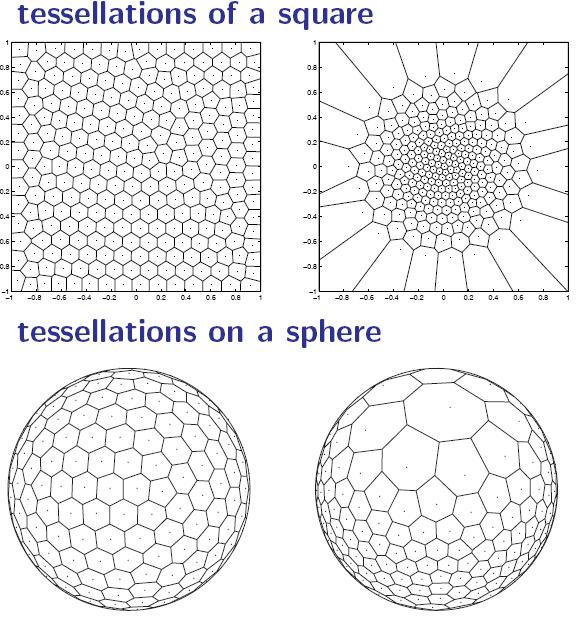
\includegraphics[width=2in]{CVTs.jpg}}
\end{columns} 
}

\subsection{Previous Method}
\frame{
\frametitle{Some Methods to construct CVTs}
\begin{itemize}
\item {\color{blue}Fixed-point iteration methods:}\\
 \qquad $\cdot$ Lloyd method (Lloyd 1960s)
\item {\color{blue}Probabilistic methods:}\\
\qquad $\cdot$ random k-means methods (Macqueen 1966)\\
\qquad $\cdot$ random 2-clustering method (Imai et.al 1994)
\item {\color{blue}Newton-based methods:}\\
\qquad $\cdot$ Newton-Lloyd method (Du/Emelianenko 2008)\\
\qquad $\cdot$ quasi-Newton L-BFGS method (Liu et.al 2009)\\
\item {\color{blue}Multigrid/multilevel methods:}\\
 \qquad $\cdot$  Lloyd-Multilevel (Du/Emelianenko 2008)\\
 \qquad $\cdot$ Multilevel Lloyd-Max (Koren/Yavneh 2003,2006)\\
\end{itemize}
}
 


\section{Introduction of MG/OPT}
\subsection{Backgroud}
\frame{
\frametitle{Introduction of MG/OPT}
\begin{itemize}
\item  MG/OPT is a {\color{blue}general} framework to accelerate a traditional optimization algorithm labeled ''OPT'', first introduced in [S.G. Nash 2000].
\vspace{.2in}
\item  Recursively use coarse problems to generate search directions for fine problems
\vspace{.2in}
\item  Inspired by multigrid for elliptic PDEs \\
\vspace{.1in}
\quad $\cdot$ highly efficient algorithm

\end{itemize}
}

\frame{
\frametitle{Notations of MG/OPT components}
\begin{itemize}
\item  {\color{blue}OPT:} a convergent optimization algorithm: \\
\vspace{.1in}
\qquad \, \, $\bz^+ \leftarrow \mbox{Opt}(\cg(\cdot),\bv,\bar \bz,k)$
\vspace{.1in}
\item {\color{blue}$h$:} fine grid; {\color{blue}$H$:} coarse grid
\vspace{.1in}
\item a high-fidelity model {\color{blue}$\cg_h$}
\vspace{.1in}
\item a low-fidelity model {\color{blue}$\cg_H$}
\vspace{.1in}
\item a downdate operator {\color{blue}$\IhH$}
\vspace{.1in}
\item an update operator {\color{blue}$\IHh$}
\end{itemize}
}

\frame{
\frametitle{Multigrid Optimization Algorithm (MG/OPT)}
\begin{itemize}
\item Given:
\begin{itemize}
\item an initial estimate $\bv_h^0 $ of the solution $\bz_h$ on the fine level
\item Integers $k_{1}$ and $k_{2}$ satisfying $k_{1}+k_{2}>0$
\end{itemize}

\item One iteration of MG/OPT:
\begin{itemize}
\item {\color{blue}{\em Pre-smoothing:}} $
\bar \bz_h \leftarrow \mbox{Opt}(\cg_h(\cdot),\bv_h,\bz_h^j,k_1)
$
\item {\color{blue}{\em Recursion:}}
\begin{itemize}
\item Compute
\begin{eqnarray*}
\zHbar &=& \IhH\zhbar \\
\vbar &=& \IhHb \bv_h + \nabla \cg_H(\zHbar) - \IhHb\nabla \cg_h(\zhbar)
\end{eqnarray*}
\item Apply MG/Opt recursively to the surrogate model:
$$
\zHplus \leftarrow
\mbox{MG/Opt}(\cg_H(\cdot),\vbar,\zHbar)
$$
\item Compute the search directions $e_H = \zHplus - \zHbar$ and $e_h = \IHh e_H$.
\item Use a line search to determine $\zhplus = \zhbar + \alpha e_h$ satisfying $\cg_h(\zhplus) \le \cg_h(\zhbar)$.
\end{itemize}
\item {\color{blue}{\em Post-smoothing:}} $
\bz_h^{j+1} \leftarrow \mbox{Opt}(\cg_h(\cdot),v_h,\bz_h^+,k_2)
$
\end{itemize}
\end{itemize}
}

\frame{
\frametitle{Properties of MG/OPT}
\begin{itemize}
\item Not dependent on a specific (single-grid) optimization algorithm 
\vspace{.2in}
\item Isolates optimization algorithm, differential equation solver, grid generation
\vspace{.2in}
\item Convergence $\&$ descent can be guaranteed
\vspace{.2in}
\item Excellent performance at initial iteration
\end{itemize}
}

\subsection{Applying MG/OPT to CVT on CVT}
\frame{
\frametitle{MG/OPT setup}
\begin{itemize}
\item We have chosen OPT to be {\color{blue}the truncated-Newton algorithm} in our experitments
\item 1-D case:
\begin{itemize}
\item Downdate from finer to coarser grid:
\begin{itemize}
\item {\color{blue}Solution restriction (injecton)}: $[\IhH v_h]^{i}=v_h^{2i},\quad i=1,2,\ldots,k/2$
\item {\color{blue}Gradient restriction (scaled full weighting)}: $[\IhHb v_h]^{i}=\frac{1}{2} v_h^{2i-1}+ v_h^{2i}+\frac{1}{2} v_h^{2i+1}, \quad i=1,2,\ldots,k/2$
\end{itemize}
\item Update from coarser to finer grid: $\IHh=(\IhHb) \tr$
\end{itemize}
\item 2-D case:
\begin{itemize}
\item Downdate from finer to coarser grid:
\begin{itemize}
\item Solution restriction is performed by {\color{blue}injection}
\item {\color{blue}Gradient restriction}: $[\IhHb v_{h}]^{i} = \sum_{j}{\alpha^i_j v_{h}^{j}}$, where $\alpha^i_i=1$ and $\alpha^i_j=\frac{1}{2}$ for any $j$ s.t. $z_j$ is a fine node sharing an edge with $z_i$ in the fine level triangulation
\end{itemize}
\item Update from coarser to finer grid: $\IHh=4(\IhHb) \tr$
\end{itemize}
\end{itemize}

}

\section{Numerical Experiments}
\subsection{1-D case}
\frame{ 
\frametitle{Convergence Result on 1-D CVT } 
\centering
 Blue: MG/Opt; Red: OPT; Green: Lloyd
\begin{columns}
\column{2.5in}
\centering
$\rho(y) = 1$ %, Circle: MG/Opt; Star: OPT; Dot: Lloyd
  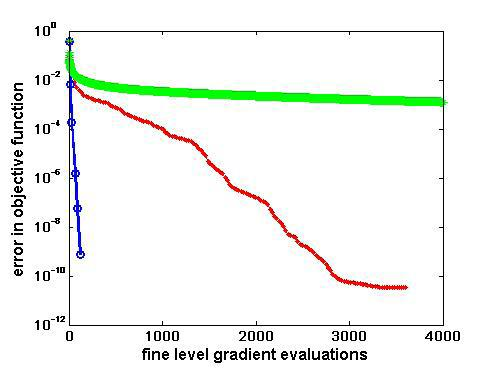
\includegraphics[width=2.5in]{valgrad512_MG_OPT_LLOYD}
\column{2.5in}
\centering
$\rho(y) = 6y^{2}e^{-2y^{3}}$
  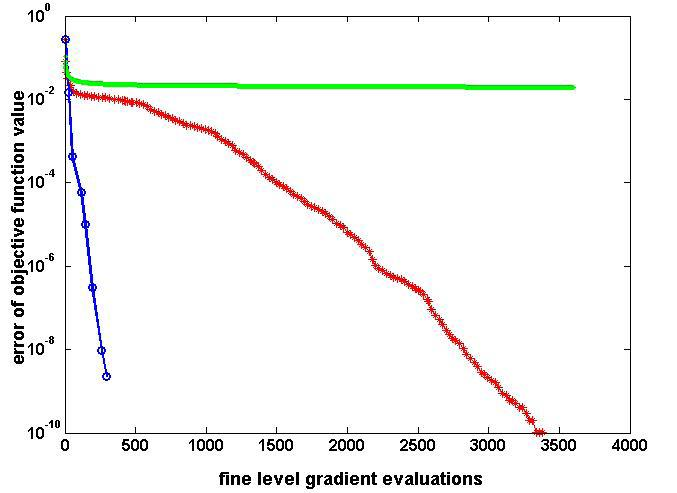
\includegraphics[width=2.5in]{nonr_512mg_opt_lloyd}
\end{columns}

}

\frame{ 
\frametitle{Convergence Result on 1-D CVT (cont'd) }
\begin{center}
Solving problems of increasing size, MG/Opt versus OPT ($\rho(y) = 1$).  Blue: MG/Opt, Red: OPT; %Cycle numbers and Time elapsed are log scaled
\end{center}
\centering
  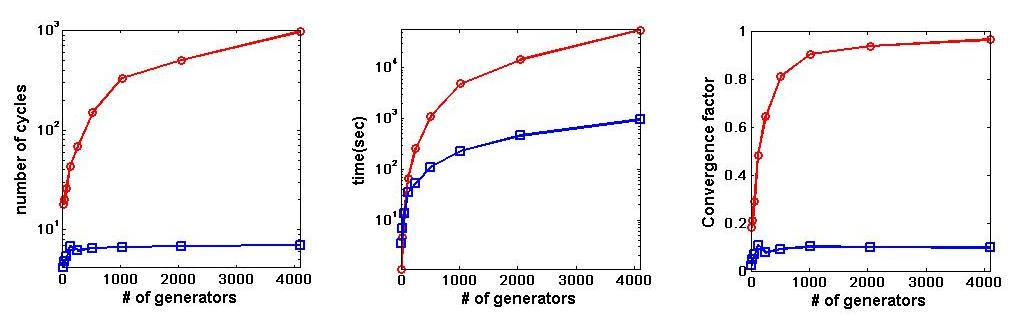
\includegraphics[width=1.0\textwidth]{ave_uni_mg_opt1.jpg}
}

\frame{ 
\frametitle{Convergence Result on 1-D CVT  (cont'd) }
\begin{center}
Performance of MG/Opt with different density functions.  Blue: $\rho(y) = 1+0.1y$.
    Red: $\rho(y) = 6y^{2} e^{-2y^{3}}$
\end{center}
\centering
  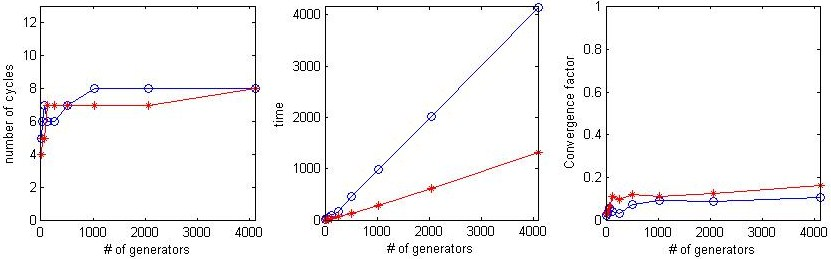
\includegraphics[width=1.0\textwidth]{diff_nonlgt}
}

\frame{ 
\frametitle{Comparison with Multilevel-Lloyd }
\begin{center}
Convergence factors for MG/Opt vs. Multilevel-Lloyd  $\rho(y) = 1$; Blue: MG/Opt; Red: Multilevel-Lloyd
\end{center}
\centering
  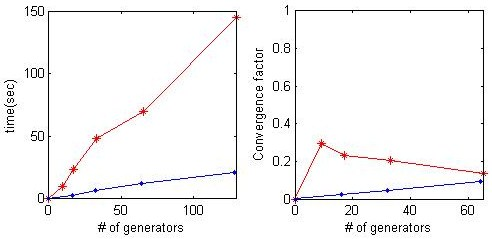
\includegraphics[width=1.0\textwidth]{uniform_mg_ml}
}

\frame{
\frametitle{Comparison with Multilevel Lloyd-Max}
\begin{table}
\begin{center}
\resizebox{10cm}{2cm} {
\begin{tabular}{| l |c | c | c | c | } \hline
 &\multicolumn{4}{|c|}{convergence factor} \\ \hline
k& ${\tt MG/Opt}^{2}$&${\tt MG/Opt}^{1}$&{\tt MLM}&{\tt OPT}\\ \hline
16&0.0350&0.0023&0.1725&0.8060\\ \hline
32&0.0314&0.0177&0.1782&0.9024 \\ \hline
64&0.0673&0.0551&0.1847&0.9381\\ \hline
128&0.1120&0.0673&0.1962&0.9736 \\ \hline
\end{tabular}
}
\end{center}
\caption{MG/OPT v.s. Multilevel Lloyd-Max v.s. OPT; density: $y=6x^{2}e^{-2x^{3}}$
\vspace{.1in}
\qquad $\ds C^{1}=\frac{|\cg(\bz^{k+1})-\cg(\bz^{*})| }{|\cg(\bz^{k})-\cg(\bz^{*})| }$;    $\ds C^{2}= \Big(\frac{|\cg(\bz^{k+1})-\cg(\bz^{*})| }{|\cg(\bz^{1})-\cg(\bz^{*})| }\Big)^\frac{1}{k+1}$}
\end{table}
}

\frame{ 
\frametitle{Convergence Result on 2-D CVT based on triangular domain }
\begin{center}
Red: Opt;   Blue: MG/OPT; $\rho(x)=1$
\end{center}
\centering
  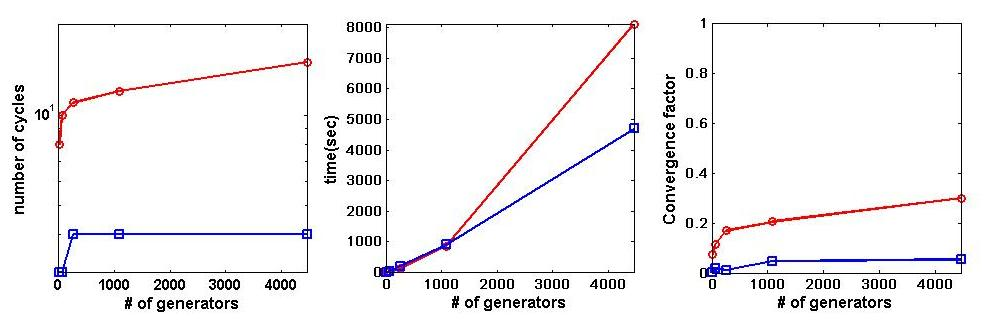
\includegraphics[width=1.0\textwidth]{comp_opt_mg_low1.jpg}
 % \caption{Comparison of performance of MG/Opt and OPT  for the case of a triangular 2-d 
 % region with $\rho=1$. Red-Circle: OPT, Blue-Square: MG/Opt.} 
{\footnotesize{ Di/Emelianenko/Nash, to appear in NMTMA, 2011}}
}

\section{Comments and Conclustions}
\frame{
\frametitle{Results and challenges}
\begin{itemize}

\item CVT is in the heart of many applications and the number is growing:\\
computer science, physics, social sciences, biology, engineering ...

\item The main advantage of MG/OPT is its superior convergence speed, and the fact that it preserves low convergence factor regardless of the problem size.

\item The simplicity of its design and the results of preliminary tests suggest that the method is generalizable to higher dimensions, which is the subject of further investigations

\item Future work also includes application of this technique to various scientific and engineering applications, including image analysis and grid generation.
\end{itemize}
\onslide<2->
{\begin{center}
\textcolor{red}{THANKS!}
\end{center}
}
}
\end{document}

